\documentclass[12pt,a4paper]{article}
\usepackage[top=2.5cm,bottom=2.5cm,left=2.2cm,right=2.2cm]{geometry}
\usepackage{polski}
\usepackage[utf8]{inputenc}
%%\usepackage[OT4]{fontenc}
\usepackage{amsmath,amsfonts,amssymb,amsthm}
\usepackage{enumerate}
\usepackage{url}
\usepackage{multicol}
\usepackage{color}
\usepackage{graphicx} 
\usepackage{setspace}
\usepackage{float}
\usepackage{subfig}
\usepackage{listings}
\usepackage{pythonhighlight}

%\pagestyle{empty}
%WYMIARY STRONY
\topmargin -30mm
\oddsidemargin -1.7cm
\evensidemargin -1.7cm
\textwidth 180mm
\textheight 260mm
%\usepackage{psfrag}

\usepackage{amsmath}
\usepackage{amsfonts}

\usepackage{supertabular}
\usepackage{array}


\usepackage{tabularx}
\usepackage{hhline}

\newcommand{\myand}{i\ }
%\usepackage{showlabels}

\newcommand{\R}{I\!\!R} %symbol liczb rzeczywistych, dzia³a tylko w
                        %trybie matematycznym
\newtheorem{theorem}{Twierdzenie}[section] %nowe otoczenie do
                                           %sk³adania twierdzeñ

\usepackage{titlesec}
\titleformat*{\section}{\normalsize\bfseries}
\titleformat*{\subsection}{\footnotesize\bfseries}
\titleformat*{\subsubsection}{\normalsize}
\title{Klasyfikator oparty na twierdzeniu Bayesa przy naiwnym założeniu o wzajemnej niezależności atrybutów}
\date{13.03.2018}
\author{Łukasz Odwrot 218283}

%ustawianie marginesów
\usepackage{geometry}
\newgeometry{tmargin=2.5cm, bmargin=2.5cm, lmargin=2.5cm, rmargin=2.5cm}


 
 
\begin{document}
\maketitle
\thispagestyle{empty}
\newpage
\tableofcontents
\setcounter{page}{1}
\newpage

\section{Wstęp}
Naiwny klasyfikator bayesowski to prosty klasyfikator probabilistyczny oparty o twierdzenie Bayesa i założeniu o niezależności zmiennych losowych.  Dla danej klasy obiektu y i wektora cech X na podstawie twierdzenia Bayesa prawdziwy jest wzór:


$$ P(y\mid x_{1},..., x_{n}) = 
\frac
{P(y)P(x_{1},...x_{n}\mid y)}
{P(x_{1},...,x_{n})}
$$

Korzystając z założenia o niezależności zdarzeń i przekształceń można dojść do wzoru:

$$  \hat{y} = arg \max_{y} P(y) \prod_{i=1}^{n} P(x_{i} \mid y) $$

Dzięki takiemu mechanizmowi na podstawie ciągu uczącego można wytrenować klasyfikator, a następnie wykorzystać go do klasyfikacji nowych obiektów. Do badania jakości uzyskanych klasyfikatorów użyte zostaną następujące mechanizmy: Confusion Matrix, ccuracy, Precision, Recall, Fscore. Badania zostaną przeprowadzone na trzech zbiorach danych: Iris, Wine oraz Diabetes.

\section{Implementacja klasyfikatora i problem wygładzania}

Na podstawie zaprezentowanych wcześniej wzorów można stwierdzić, że w przypadku, gdy dana kombinacja cechy  i wartości nie wystąpi w zbiorze uczącym, wyzeruje ona prawdopodobieństwo klasyfikacji do danej klasy przy wystąpieniu cechy w czasie klasyfikacji właściwej. Z tym zjawiskiem można poradzić sobie poprzez wygładzenie danych, czyli eliminację zerowych prawdopodobieństw lub założenie, że dane mają rozkład normalny. W tym wypadku można skorzystać ze wzoru, który likwiduje zerowe prawdopodobieństwa.

$$ 
P(x_{i} \mid y) = 
\frac
{1}
{\sqrt{2 \pi \sigma^{2}_{y}}}
\exp
(- 
\frac
{(x_{i} - \mu_{y})^2)}
{2\sigma^{2}_{y}}
)
$$

Do badań wykorzystane zostaną dwie implementacje pochodzące z biblioteki \emph{sklearn}: \emph{GaussianNB} oraz \emph{MultinomialNB} ze współczynnikiem wygładzania  $\alpha$ = 1, który wykorzystuje \emph{wygładzanie laplace}.

\begin{python}
def getClassifireNormal(_features, _targets):
    gnb = GaussianNB()
    gnb.fit(_features, _targets)
    return gnb

def getClassifireSmooth(_features, _targets):
    gnbM = MultinomialNB(alpha=1.0)
    gnbM.fit(_features, _targets)
    return gnbM
\end{python}

\section{Metody dyskretyzacji}
Jednym z celów zadania jest zbadanie wpływu dyskretyzacji danych na jakość klasyfikatora. W programie zaimplementowany zostały trzy rodzaje dyskretyzacji.
\begin{enumerate}
\item \emph{Equal width intervals}: podział zakresu wartości atrybutu ciągłego na k przedziałów o jednakowej szerokości.
\begin{python}
def discretizationEqualWidth(_data, _parts):
    print('Equal width')
    minMaxVals = np.array([])
    transposedData = np.array(_data[:]).transpose()
    resultData = []

    for featureVector in transposedData:
        resultData.append(
            np.digitize(
                featureVector,
                np.linspace(min(featureVector), max(featureVector), _parts)
            )
        )

    resultData = np.array(resultData).transpose()
    return resultData
\end{python}
\item \emph{Equal frequency intervals }: podział zakresu wartości atrybutu ciągłego na   przedziałów, z których każdemu odpowiada możliwie tyle samo przykładów ze zbioru trenującego.
\begin{python}

def discretizationEqualFreq(_data):
    print('Equal freq')
    groups = 10
    orangeTable = Orange.data.Table(_data)
    disc = Orange.preprocess.Discretize()
    disc.method = Orange.preprocess.discretize.EqualFreq(n=groups)
    orangeDiscrete = disc(orangeTable)
    mSets = [set() for i in range(0, len(_data[0]))]
    for sample in orangeDiscrete:
        for index in range(0, len(sample)):
            numbers = [float(s) for s in str(sample[index]).split() if is_number(s)]
            for numb in numbers:
                mSets[index].add(numb)

    # create bins
    mBins = []
    for mSet in mSets:
        mBins.append(sorted(list(mSet)))


    transposedData = np.array(_data[:]).transpose()
    resultData = []
    for index, featureVector in enumerate(transposedData):
        resultData.append(
            np.digitize(
                featureVector,
                mBins[index]
            )
        )

    resultData = np.array(resultData).transpose()
    return resultData
\end{python}

\item \emph{Quantile transform}: konwersja danych do postaci rozkładu normalnego i przypisanie dyskretnych wartości, użyta zostanie funkcja dostępna w pakiecie sklearn.
\begin{python}
def discretizationQuantileTransform(_data, _quantiles=100):
    print('Quantile')
    nData = list(_data)
    return quantile_transform(nData, n_quantiles=_quantiles, random_state=0) 
\end{python}
\end{enumerate}

Działanie poszczególnych metod dyskretyzacji dla instancji Iris przedstawiono poniżej.

\begin{figure}[H]
\centering
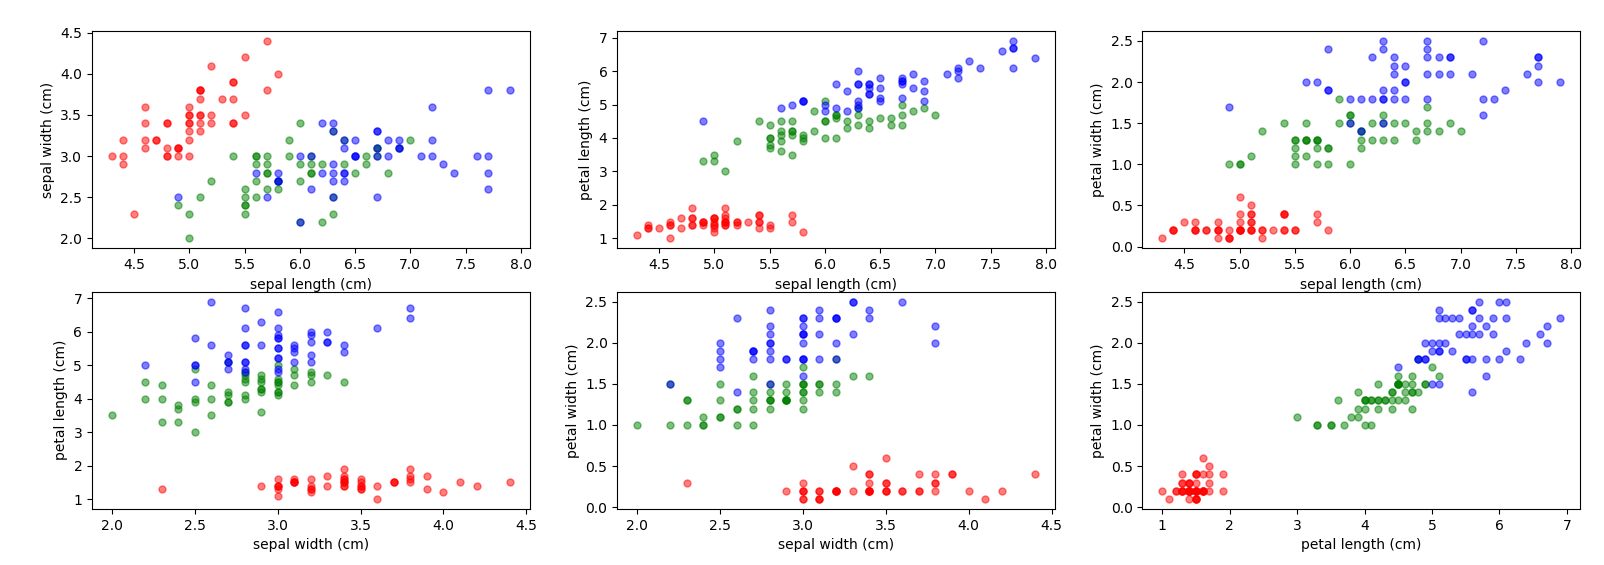
\includegraphics[width=1\textwidth]{discretization_none.PNG}
\caption{Brak dyskretyzacji}
\end{figure}

\begin{figure}[H]
\centering
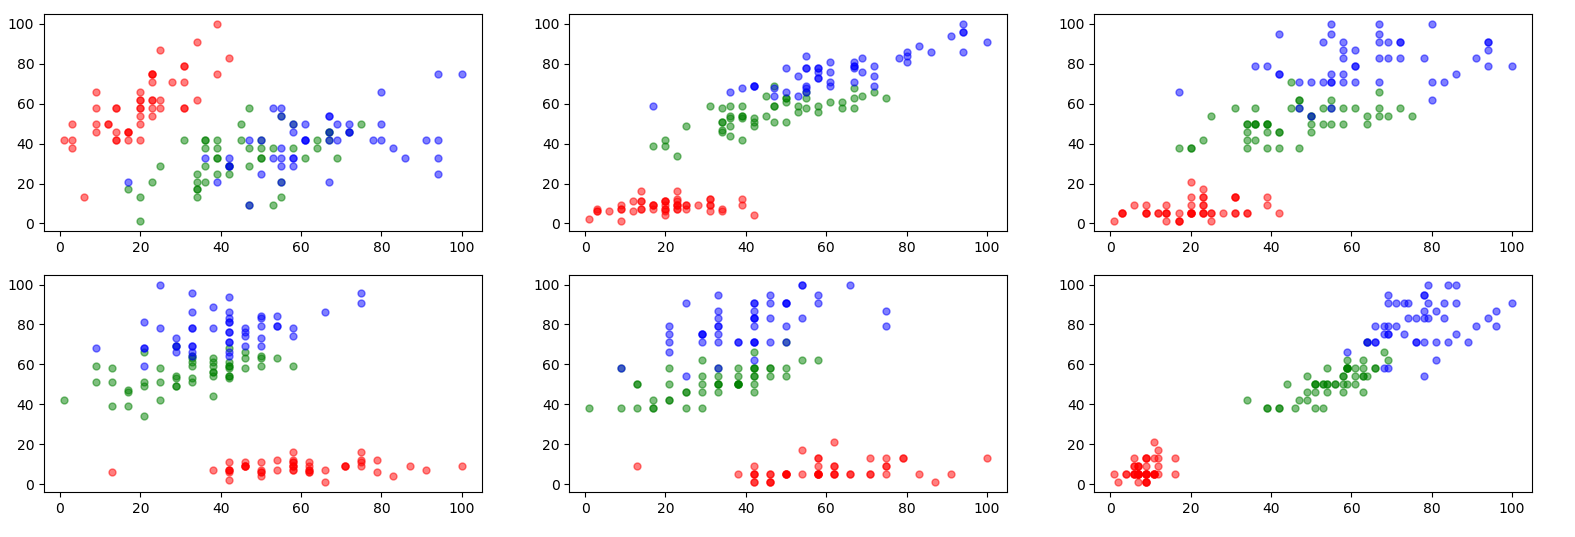
\includegraphics[width=1\textwidth]{discretization_equalWidth.PNG}
\caption{Equal width (100 intervals)}
\end{figure}


\begin{figure}[H]
\centering
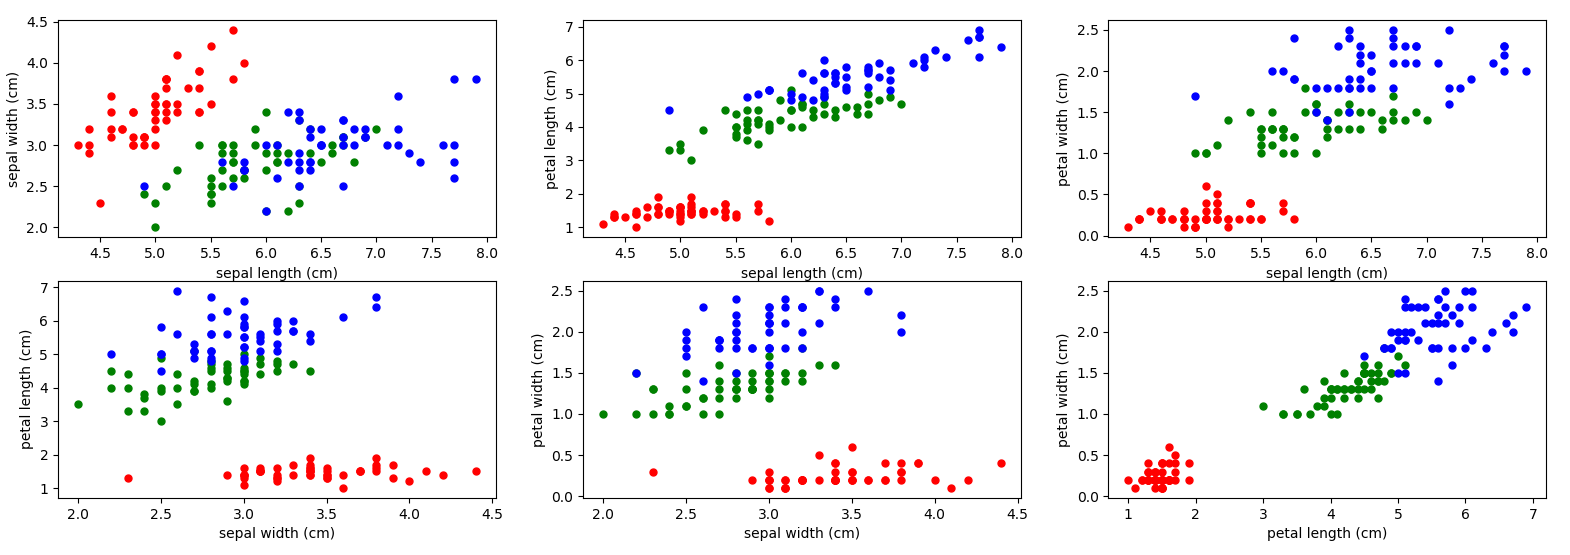
\includegraphics[width=1\textwidth]{discretization_quantile.PNG}
\caption{Quantile transform}
\end{figure}

\section{Wybór instancji}
Do testów wykorzystane zostaną gotowe zbiory danych: iris, wine oraz diabetes. Każdy z nich posiada inną ilość cech, które będą uwzględniane w procesie klasyfikacji. Instancje przedstawione zostały na poniższych rysunkach.

\begin{figure}[H]
\centering
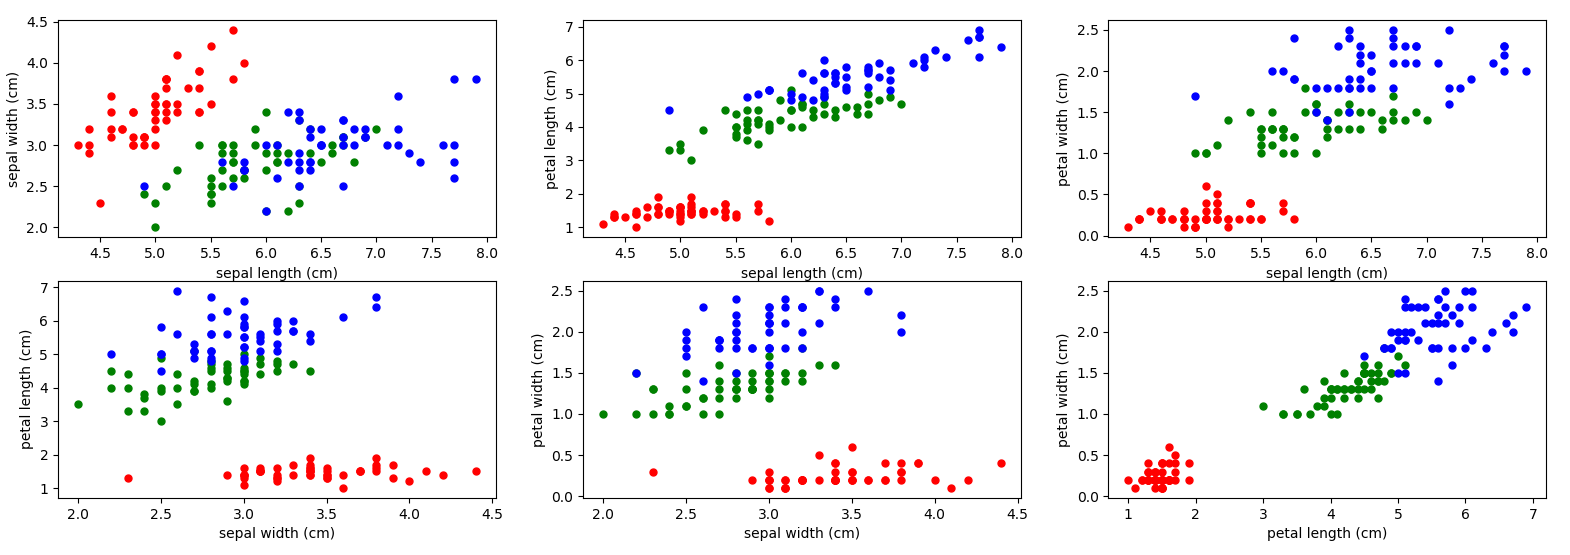
\includegraphics[width=1\textwidth]{irisData.PNG}
\caption{Instancja Irir}
\end{figure}

\begin{figure}[H]
\centering
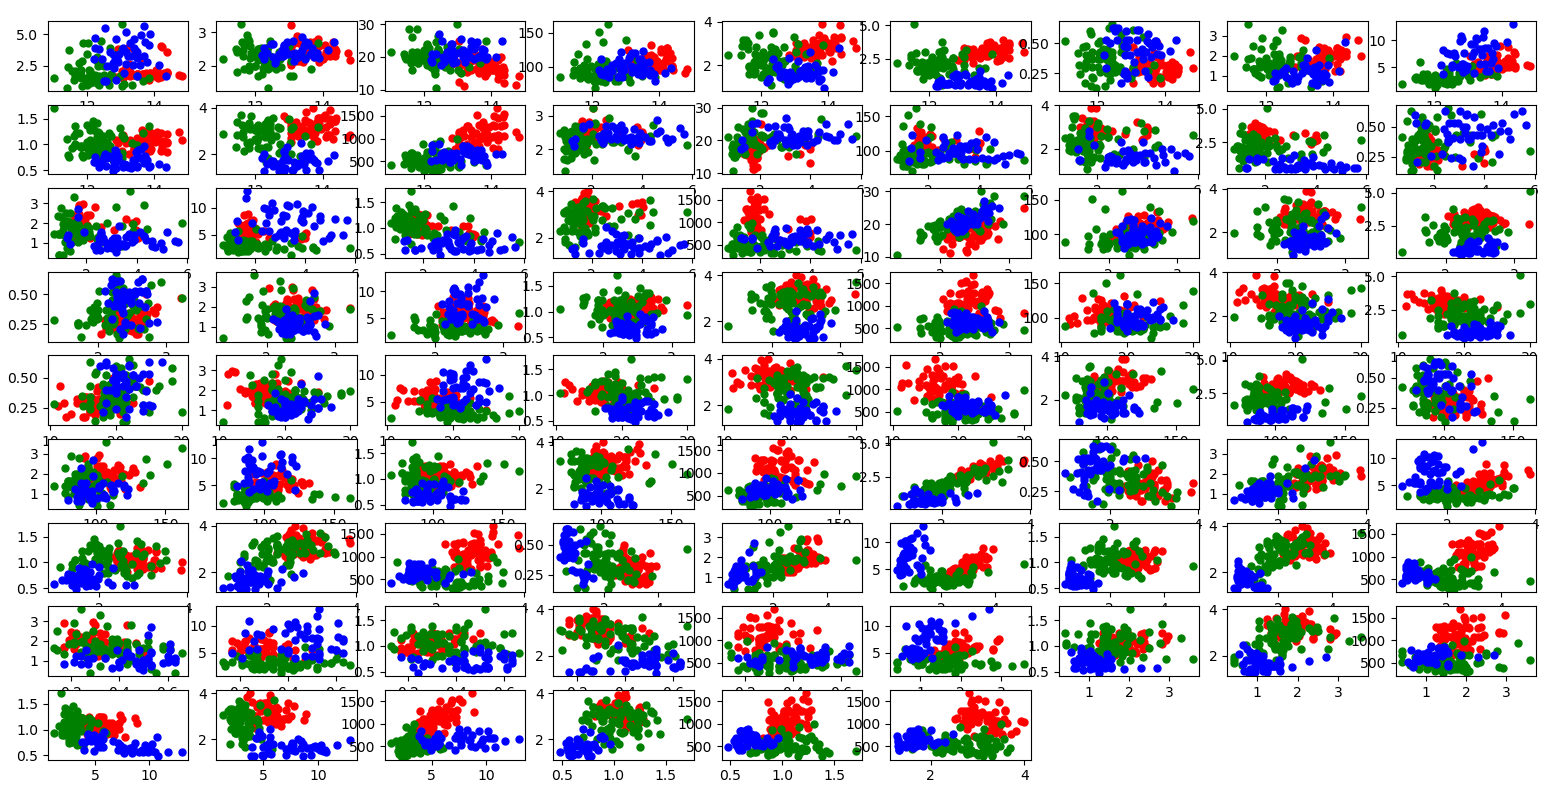
\includegraphics[width=1\textwidth]{wineData.PNG}
\caption{Instancja Wine}
\end{figure}

\begin{figure}[H]
\centering
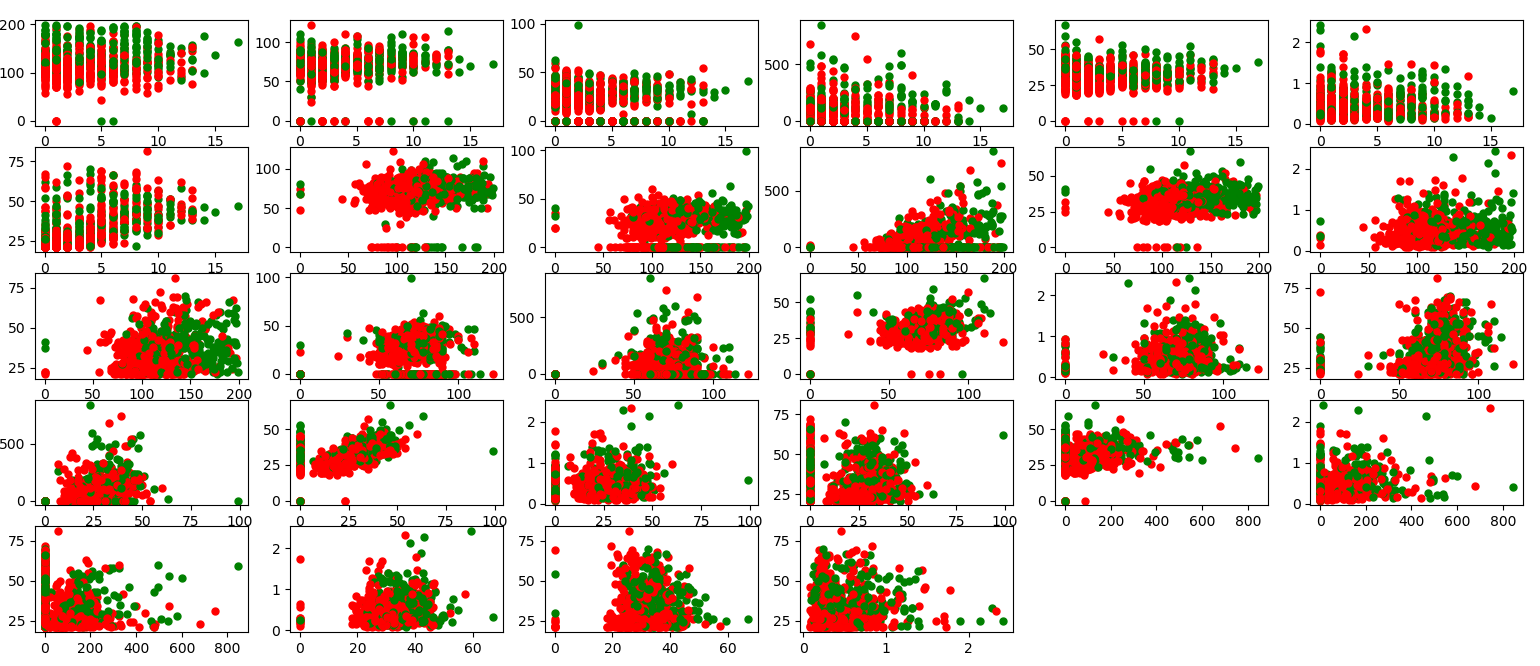
\includegraphics[width=1\textwidth]{diabetesData.PNG}
\caption{Instancja Diabetes}
\end{figure}


\section{Porównanie działania algorytmu przy różnych podziałach danych i sposobie liczenia prawdopodobieństwa}
Do oceny klasyfikatora zostanie użyta metoda kroswalidacji z metodą podziału \emph{X-fold}. Polega ona na tym, że zbiór dzielimy na X w miarę możliwości równych części. Każda część zawiera możliwie tyle samo danych z każdej klasy. Jedna część zostanie użyta do oceny klasyfikatora, a pozostałe wejdą w skład zbioru trenującego. Następnie X razy zmianie ulegnie część do klasyfikacji, a cały proces zostanie powtórzony. 
Przetestowana zostanie metoda uczenia poprzez podział zbioru na 3, 5 i 10 części. Ponadto sprawdzone zostaną dwie metody liczenia prawdopodobieństwa – \emph{Gausian} oraz \emph{Multinomial} z wygładzaniem laplaca.

\begin{figure}[H]
\centering
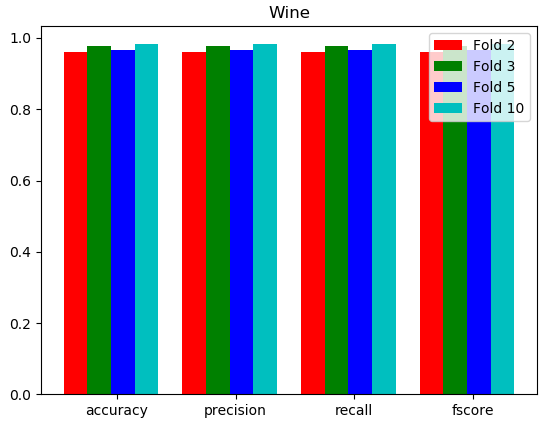
\includegraphics[width=0.8\textwidth]{gMeasure.PNG}
\caption{Współczynniki dokładności klasyfikatora dla klasyfikatora Gausian}
\end{figure}

\begin{figure}[H]
\centering
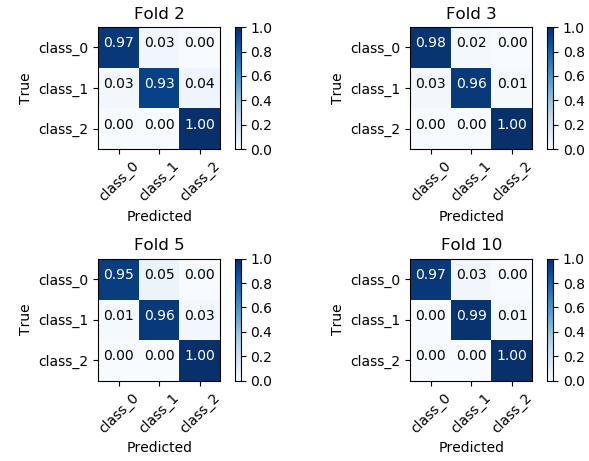
\includegraphics[width=0.8\textwidth]{gConfusion.PNG}
\caption{Confusion Matrix dla klasyfikatora Gausian}
\end{figure}

\begin{figure}[H]
\centering
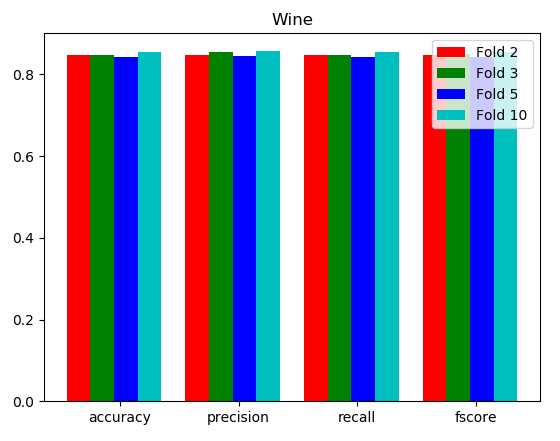
\includegraphics[width=0.8\textwidth]{mMeasure.PNG}
\caption{Współczynniki dokładności klasyfikatora dla klasyfikatora Multinomial}
\end{figure}

\begin{figure}[H]
\centering
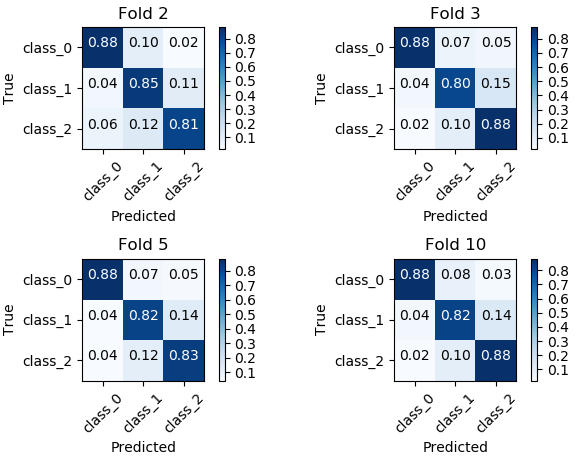
\includegraphics[width=0.8\textwidth]{mConfusion.PNG}
\caption{Confusion Matrix dla klasyfikatora Multinomial}
\end{figure}

Można zauważyć, że zmiana ilości podziałów nie ma wpływu na wynik klasyfikacji, co jest spowodowane rozkładem badanych danych. Natomiast zmiana metody liczenia prawdopodobieństwa na sprawiła, że wyniki klasyfikatora uległy znaczącemu pogorszeniu.
W późniejszych eksperymentach użyta zostanie metoda 10-fold do walidacji oraz Gausian do liczenia prawdopodobieństwa.  


\section{Porównanie działania metod dyskretyzacji dla badanych zbiorów}
Zaimplementowany klasyfikator zostanie użyty na wybranych wcześniej zbiorach. Dla każdego z nich porównane zostaną wyniki otrzymane przy użyciu różnych metod dyskretyzacji danych. Wyniki przedstawiono na poniższych rysunkach.

\begin{figure}[H]
\centering
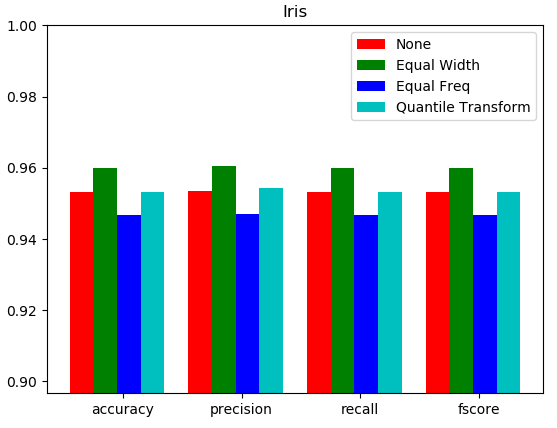
\includegraphics[width=0.8\textwidth]{tsIris.PNG}
\caption{Współczynniki dokładności klasyfikatora dla zbioru Iris}
\end{figure}

\begin{figure}[H]
\centering
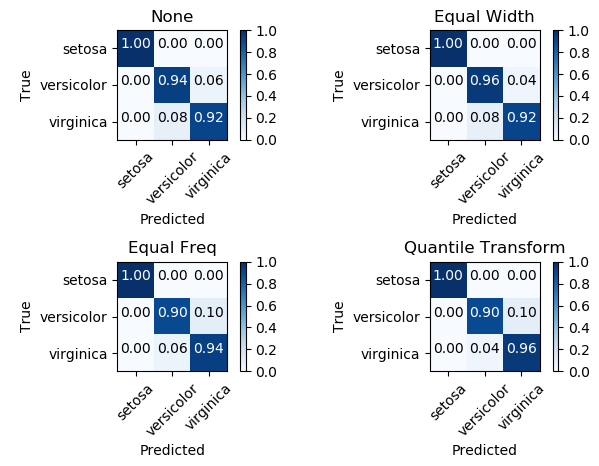
\includegraphics[width=0.8\textwidth]{tmIris.PNG}
\caption{Confusion Matrix dla zbioru Iris}
\end{figure}

\begin{figure}[H]
\centering
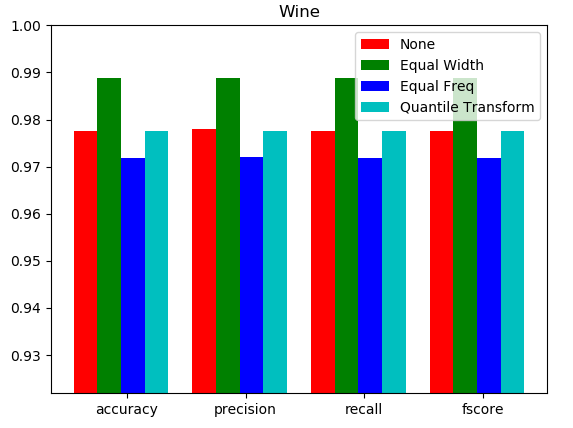
\includegraphics[width=0.8\textwidth]{tsWine.PNG}
\caption{Współczynniki dokładności klasyfikatora dla zbioru Wine}
\end{figure}

\begin{figure}[H]
\centering
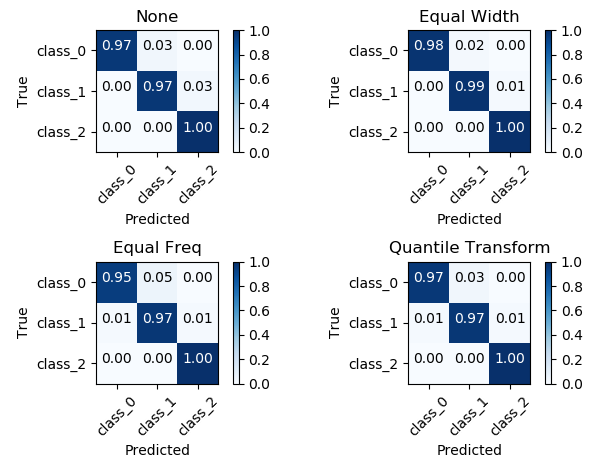
\includegraphics[width=0.8\textwidth]{tmWine.PNG}
\caption{Confusion Matrix dla zbioru Wine}
\end{figure}

\begin{figure}[H]
\centering
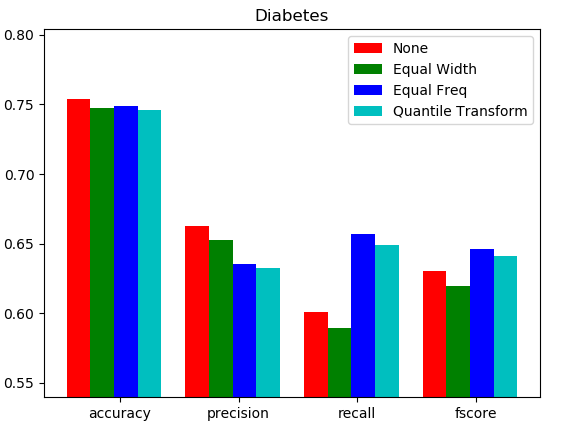
\includegraphics[width=0.8\textwidth]{tsDiabetes.PNG}
\caption{Współczynniki dokładności klasyfikatora dla zbioru Diabetes}
\end{figure}

\begin{figure}[H]
\centering
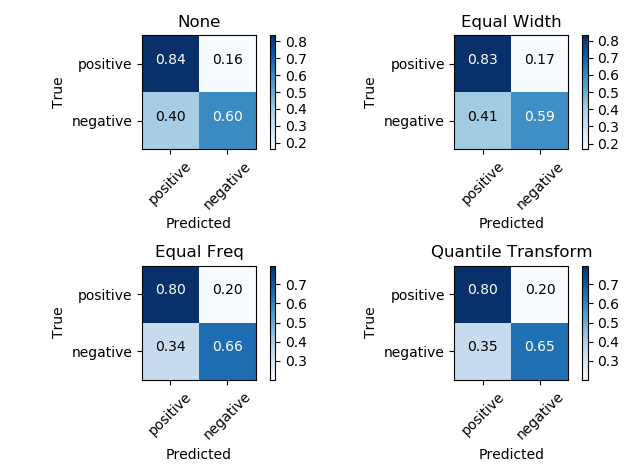
\includegraphics[width=0.8\textwidth]{tmDiabetes.PNG}
\caption{Confusion Matrix dla zbioru Diabetes}
\end{figure}

Pomimo zupełnie innych metod dyskretyzacji, jakość klasyfikatorów nie różni się znacząco. W przypadku zbioru \emph{Wine} widać, że najlepsze wyniki osiągnęła metoda równomiernego podziału, ale nie jest to znacząca różnica. W pozostałych przypadkach ciężko jednoznacznie określić najlepszą metodę dyskretyzacji.
\section{Wnioski}
W ramach zadania zaimplementowany został naiwny klasyfikator bayesa. Przyjęcie, że cechy wybranych zbiorów mają rozkład Gausa dało o wiele lepsze wyniki niż użycie mechanizmu MultinomialBayes. Niezależnie od wykorzystanej metody dyskretyzacji uzyskane klasyfikatory rozpoznawały obiekty ze zbliżoną precyzją. Jest to związane z rozkładem cech danych dla badanych zbiorów.

\end{document}





























